\documentclass[tikz]{standalone}

% mytikzset
\usepackage{tikz}
\usetikzlibrary{positioning,arrows,shapes,patterns}
\usetikzlibrary{decorations.pathmorphing}
\usetikzlibrary{decorations.pathreplacing}
\usetikzlibrary{decorations.markings}
\usetikzlibrary{shapes.arrows, fadings}
\usetikzlibrary{calc}
\usetikzlibrary{}


\tikzset{
  vector/.style={thick,double,draw=black, postaction={decorate},
    decoration={markings,mark=at position .6 with {\arrow[black,scale=0.4]{triangle 45}}}},
  axial/.style={thick,double,densely dashed,draw=black, postaction={decorate},
    decoration={markings,mark=at position .6 with {\arrow[black,scale=0.4]{triangle 45}}}},
  gluon/.style={decorate, draw=black,
    decoration={coil,aspect=0.3,segment length=5pt,amplitude=3pt}},
  pseudo/.style={thick, dashed, draw=black, postaction={decorate},
    decoration={markings,mark=at position .6 with {\arrow[red,scale=0.5]{triangle 45}}}},
  scalar/.style={thick,draw=black, postaction={decorate},
    decoration={markings,mark=at position .6 with {\arrow[black,scale=0.5]{triangle 45}}}}%,
  % pomeron/.style={thick,draw=black, postaction={decorate},
  % decoration={zigzag,segment length=4,amplitude=.9}}
}

\definecolor{myGreen}{RGB}{0,127,0}

\begin{document}
\nopagecolor
  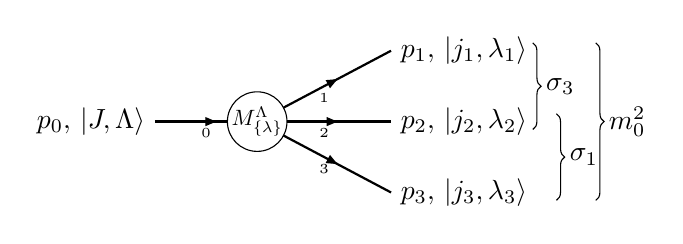
\begin{tikzpicture}[node distance=0.9cm and 1.3cm, baseline=1cm]
    \coordinate[] (c0);
    \coordinate[left=of c0,label= left:{$p_0,\,\left|J,\Lambda\right\rangle$}] (Lamc);
    \coordinate[above right=of c0, xshift=4mm, label=right:{$p_1,\,\left|j_1,\lambda_1\right\rangle$}] (p);
    \coordinate[ right=of c0, xshift=4mm, label=right:{$p_2,\,\left|j_2,\lambda_2\right\rangle$}] (K);
    \coordinate[below right=of c0, xshift=4mm, label=right:{$p_3,\,\left|j_3,\lambda_3\right\rangle$}] (pi);

    \draw[scalar]  (Lamc) -- node[yshift=-1.5mm] {\tiny $0$}  (c0);
    \draw[scalar]  (c0) -- node[yshift=-1.5mm] {\tiny $1$} (p);
    \draw[scalar]  (c0) -- node[yshift=-1.5mm] {\tiny $2$} (K);
    \draw[scalar]  (c0) -- node[yshift=-1.5mm] {\tiny $3$} (pi);

    \draw[black, fill=white] (c0) circle (2.5ex) node[scale=0.8] {$M^{\Lambda}_{\{\lambda\}}$};

    \draw [decorate,decoration={brace,amplitude=3pt}] ($(p)+(1.8,0.1)$) -- ($(K)+(1.8,-0.1)$) node [black,midway,xshift=0.35cm] {$\sigma_3$};
    \draw [decorate,decoration={brace,amplitude=3pt}] ($(K)+(2.1,0.1)$) -- ($(pi)+(2.1,-0.1)$) node [black,midway,xshift=0.35cm] {$\sigma_1$};
    \draw [decorate,decoration={brace,amplitude=3pt}] ($(p)+(2.6,0.1)$) -- ($(pi)+(2.6,-0.1)$) node [black,midway,xshift=0.4cm] {$m_0^2$};

  \end{tikzpicture}
\end{document}
